\section{Introduction}



%%%%%%%%%%%%%%%%%%%%%%%%%%%%%%%%%%%%%%%%%%%%%%%%%%%%%%%%%%%%%%%%%%%%%%%%%%%%%%%
\section{Methodology}

The methodology proposed by \citet{Souza-Junior2023b} aimed to achieve the semi-automatic estimation of dipole moments for individual grains per image. This is approached through a three-part methodology. The initial step involves the application of classic potential field data processing, such as total gradient amplitude, coupled with image processing techniques like histogram stretching, equalization, and an edge detection algorithm. This enables the identification and spatial isolation of the magnetic field caused by each source. 

Following that, attention shifts to the estimation of the 3D position of magnetic particles based on magnetic field measurements. This is carried out by applying the Euler deconvolution method to the data segment identified in the first step. In the final phase, the magnetic moment inversion process is executed. This entails estimating the 3-component dipole moment vector by inverting the magnetic field data assuming a dipolar model. The inversion is conducted separately for each data segment identified initially, which in theory ensures stability and computational efficiency in solving the linear inverse problem in a few seconds. 

However, estimating the source's position based on Euler deconvolution revealed that stronger magnetic sources may influence the estimated positions of nearby weaker ones. Therefore, it becomes imperative to consider the interplay among the sources to estimate their magnetic parameters and position accurately. Understanding how these magnetic sources interact with each other is crucial for refining our estimation process and ensuring robust results in magnetic parameter estimation.

\subsection{Magnetic inversion: interfering sources}
    
% This study explores three distinct methods for handling interfering sources during inversion. The first approach involves employing the interactive Euler deconvolution method, where interference from other sources is systematically removed in each window. The second method considers interference using the $b_z$ vector, in which the inversion is performed on the entire set of particles. Lastly, we explore a similar approach as the second method but applied to the first derivative of $b_z$.

This study explores methodologies to effectively manage interfering sources during the inversion process. In the following sections, three distinct methodologies are presented, each designed to mitigate the magnetic sources' interference and enhance the precision of the inversion analyses proposed by \citet{Souza-Junior2023b}.


% Accurate results in geophysical investigations heavily depend on overcoming the challenges posed by concurrent magnetic signals. 



% \begin{enumerate}
%     \item \textbf{Interactive Euler Deconvolution Method:}
%     \begin{itemize}
%         \item Systematically removes interference from other sources within specific windows during the inversion process.
%     \end{itemize}
    
%     \item \textbf{$b_z$ Vector Method:}
%     \begin{itemize}
%         \item Addresses interference through the magnetic induction vector \(b_z\). The inversion is applied to the entire set of particles, ensuring a comprehensive consideration of interference in the dataset.
%     \end{itemize}
    
%     \item \textbf{First Derivative of $b_z$ Method:}
%     \begin{itemize}
%         \item Variant of the second method, involving the application of inversion to the first derivative of \(b_z\). This provides an alternative means to handle interference while enhancing the accuracy of the inversion process.
%     \end{itemize}
% \end{enumerate}



\subsubsection{Iteractive Euler deconvolution}

The first proposed methodology aims to enhance the accuracy of inversion analyses in magnetic data, particularly in scenarios where stronger magnetic sources may distort the results. The process is divided into distinct steps:

\begin{enumerate}
  \item \textbf{Automatic Source Detection:} Utilizing edge detection on the total gradient amplitude (TGA), the algorithm identified and segmented window data of the magnetic sources in descending order of magnitude (blob intensity). 

  \item \textbf{Position Estimation:} Subsequently, the Euler deconvolution was applied in the window data to obtain a 3D position estimation.
  
  \item \textbf{Calculation of Theoretical Magnetic Signals:} The theoretical magnetic signal associated with the identified source was computed using a dipole forward model with the aid of Choclo python library \citep{choclo2022}. This yielded a theoretical representation of the expected magnetic effects from each source.
  
  \item \textbf{Signal Removal:} The magnetic signal from the strong source, computed in the previous step, is selectively removed from the dataset. This leads to a dataset that is devoid of the strong source's dominant influence, allowing for a gradual isolation of the contributions from weaker sources. The directional derivatives were also recalculated in order to re-calibrate the next Euler deconvolution within this updated dataset.
    
  % The magnetic signal attributed to the strong source, calculated in the previous step, is selectively removed from the dataset. Resulting in a dataset, now devoid of the dominant effect of the strong source, that progressively isolates the contributions of weaker sources. In the updated dataset, we also recalculate all directional derivatives required in the Euler deconvolution.
\end{enumerate}

This step-by-step procedure is subsequently employed for all detected particles in the sample, leading to an improved position estimation compared to the previous analyses. Designed to mitigate the impact of stronger sources and with a better estimation of positions, this method significantly enhances the precision of subsequent inversion analyses. Although, a trade-off between achieving better results and incurring longer computational runtime is unavoidable. 



%%%%%%%%%%%%%%%%%%%%%%%%%%%%%%%%%%%%%%%%%%%%%%%%%%%%%%%%%%%%
\subsubsection{Vertical component magnetic field ($\mathbf{b_z}$)}\label{section_bz}
After identifying the position of the source, assuming it is a dipole, we can utilize the modified approach from \citet{Oliveira2015Estimation} to calculate the dipole moment vector, denoted as 
\textbf{m}. The magnetic induction vector $\mathbf{b_z}$ for a dipole is given by

\begin{equation}
\label{eq_dipole_bz}
\mathbf{b_z}
= \dfrac{\mu_0}{4\pi}
\begin{bmatrix}
\dfrac{\partial^2}{\partial z \partial x} \dfrac{1}{r}
& \dfrac{\partial^2}{\partial z \partial y} \dfrac{1}{r}
& \dfrac{\partial^2}{\partial z \partial z} \dfrac{1}{r}
\end{bmatrix}
\begin{bmatrix}
m_x \\ m_y \\ m_z
\end{bmatrix}
= \dfrac{\mu_0}{4\pi} \mathbf{M_z}\,\mathbf{m}
\ .
\end{equation}

To address the mutual interference of magnetic sources, a method involves simultaneously solving the magnetic moment inversion for all "L" identified, therefore the Equation \ref{eq_dipole_bz} becomes


\begin{equation}
% \footnotesize
\label{eq_dipole_bz_all}
\dfrac{\mu_0}{4\pi}
{\begin{bmatrix}
\dfrac{\partial^2}{\partial z \partial x} \dfrac{1}{r_{1,1}}
& \dfrac{\partial^2}{\partial z \partial y} \dfrac{1}{r_{1,1}}
& \dfrac{\partial^2}{\partial z \partial z} \dfrac{1}{r_{1,1}}
& \hdots
& \dfrac{\partial^2}{\partial z \partial x} \dfrac{1}{r_{1,L}}
& \dfrac{\partial^2}{\partial z \partial y} \dfrac{1}{r_{1,L}}
& \dfrac{\partial^2}{\partial z \partial z} \dfrac{1}{r_{1,L}} \\
\\

& 
& 
& \vdots
& 
& 
&  \\
\\
\dfrac{\partial^2}{\partial z \partial x} \dfrac{1}{r_{N,1}}
& \dfrac{\partial^2}{\partial z \partial y} \dfrac{1}{r_{N,1}}
& \dfrac{\partial^2}{\partial z \partial z} \dfrac{1}{r_{N,1}}
& \hdots
& \dfrac{\partial^2}{\partial z \partial x} \dfrac{1}{r_{N,L}}
& \dfrac{\partial^2}{\partial z \partial y} \dfrac{1}{r_{N,L}}
& \dfrac{\partial^2}{\partial z \partial z} \dfrac{1}{r_{N,L}} \\
\end{bmatrix}}_{N \times 3L}
{\begin{bmatrix}
{m_x}_1 \\ {m_y}_1 \\ {m_z}_1 \\ \vdots \\{m_x}_L \\ {m_y}_L \\ {m_z}_L \\
\end{bmatrix}}_{3L \times 1}
=
{\begin{bmatrix}
{b_z}_1 \\ {b_z}_2 \\ {b_z}_3 \\ \vdots \\{b_z}_N 
\end{bmatrix}}_{N \times 1}.
\end{equation} \bigskip

In which $r_{i,j} = \sqrt{(x_i - {x_c}_j)^2 + (y_i - {y_c}_j)^2 + (z_i - {z_c}_j)^2}$ is the Cartesian distance between the i-th, $i=1, 2, \hdots N$, observation point $b_z (x_i, y_i, z_i)$ and the j-th, $j=1, 2, \hdots L$, point source $({x_c}_j, {y_c}_j, {z_c}_j)$ and $\mu_0$ is the vacuum magnetic permeability. While the three second-order derivatives in Equation~\ref{eq_dipole_bz_all} are:

\begin{equation}
% \footnotesize
\begin{aligned}
\dfrac{\partial^2}{\partial z \partial x} \dfrac{1}{r_{i,j}} &=
\dfrac{3(z_i - {z_c}_j)(x_i - {x_c}_j)}{{r_{i,j}}^5}\ ,
\\
\dfrac{\partial^2}{\partial z \partial y} \dfrac{1}{r_{i,j}} &=
\dfrac{3(z_i - {z_c}_j)(y_i - {y_c}_j)}{{r_{i,j}}^5}\ ,
\\
\dfrac{\partial^2}{\partial z \partial z} \dfrac{1}{r_{i,j}} &=
\dfrac{3(z_i - {z_c}_j)^2}{{r_{i,j}}^5} - \dfrac{1}{{r_{i,j}}^3}\ .
\end{aligned}
\end{equation}   \bigskip

The Equation \ref{eq_dipole_bz_all} can be expressed in matrix form as

\begin{equation}
\label{qdhqM4s9Ln}
\mathbf{M_z} \mathbf{m} = \mathbf{b_z}^{pred} \ .
\end{equation}

The dipole moment vector that best fits
a set of $N$ observations of the vertical component of the magnetic field
$\mathbf{b_z}^{obs}$ is given by minimizing the misfit function using a least-squares estimator

\begin{equation}
\label{uV9pRVYO4l}
\Phi (\mathbf{m}) = \| \mathbf{b_z}^{obs} - \mathbf{b_z}^{pred} \|^2 = (\mathbf{b_z}^{obs} - \mathbf{M_z}\mathbf{m})^T  (\mathbf{b_z}^{obs} - \mathbf{M_z}\mathbf{m})\ .
\end{equation}

The dipole moment vector that minimizes $\Phi (\mathbf{m})$ can be found by solving the linear equation system

\begin{equation}
 \mathbf{m} = {\left ( \mathbf{M_z}^T \mathbf{M_z} \right )}^{-1} \mathbf{M_z}^T\mathbf{b_z}^{obs}\ .
\end{equation}

Therefore, taking into account all their mutual signal interference in the N observed data increases further the trade-off between accuracy and run time.



\subsubsection{Vertical derivative of $\mathbf{b_z}$}

%An alternative method to enhance the inversion process involves utilizing the first derivative of \( b_z \). 

Applying derivatives in geophysical investigations offers improved sensitivity to shallow sources, enabling the isolation and detailed analysis of local geological features. The flexibility and versatility inherent in fractional order derivatives allow for precise adjustments in the separation process, enabling accurate estimation of the local field, such as shown by \citet{Florio2022}. In the latter, the vertical derivative serves as a straightforward and stable tool for regional-residual separation, even in regions with restricted spatial extent. This contributes to the precise prediction and isolation of local field characteristics. 

We obtained the partial derivative ($\partial_z f$) of the magnetic field ($f$) with respect to $z$ using a second-order accurate central finite-difference scheme based on two upward continuation applications

\begin{equation}
\partial_z f(x, y, z) \approx
\dfrac{f(x + \Delta z, y, z) - f(x - \Delta z, y, z)}{2 \Delta z}
\ .
\end{equation}

This derivative functions as a high-pass filter, effectively reducing the potential interference caused by the long-wavelength signal of the stronger source with weaker sources. We can obtain \( \frac{b_z}{\partial z} \) by differentiating both sides of Equation~\ref{eq_dipole_bz_all} with respect to \( z \):



\begin{equation}
\footnotesize
\label{eq_dipole_bz_z_deriv}
\dfrac{\mu_0}{4\pi}
% \scriptsize
{\begin{bmatrix}
\dfrac{\partial^2}{\partial z \partial x \partial z} \dfrac{1}{r_{1,1}}
& \dfrac{\partial^2}{\partial z \partial y \partial z} \dfrac{1}{r_{1,1}}
& \dfrac{\partial^2}{\partial z \partial z \partial z} \dfrac{1}{r_{1,1}}
& \hdots
& \dfrac{\partial^2}{\partial z \partial x \partial z} \dfrac{1}{r_{1,L}}
& \dfrac{\partial^2}{\partial z \partial y \partial z} \dfrac{1}{r_{1,L}}
& \dfrac{\partial^2}{\partial z \partial z \partial z} \dfrac{1}{r_{1,L}} \\
\\

& 
& 
& \vdots
& 
& 
&  \\
\\
\dfrac{\partial^2}{\partial z \partial x \partial z} \dfrac{1}{r_{N,1}}
& \dfrac{\partial^2}{\partial z \partial y \partial z} \dfrac{1}{r_{N,1}}
& \dfrac{\partial^2}{\partial z \partial z \partial z} \dfrac{1}{r_{N,1}}
& \hdots
& \dfrac{\partial^2}{\partial z \partial x \partial z} \dfrac{1}{r_{N,L}}
& \dfrac{\partial^2}{\partial z \partial y \partial z} \dfrac{1}{r_{N,L}}
& \dfrac{\partial^2}{\partial z \partial z \partial z} \dfrac{1}{r_{N,L}} \\
\end{bmatrix}}_{N \times 3L}
{\begin{bmatrix}
{m_x}_1 \\ {m_y}_1 \\ {m_z}_1 \\ \vdots \\{m_x}_L \\ {m_y}_L \\ {m_z}_L \\
\end{bmatrix}}_{3L \times 1}
=
{\begin{bmatrix}
\frac{{b_z}_1}{ \partial z} \\ \frac{{b_z}_2}{ \partial z} \\ \frac{{b_z}_3}{ \partial z} \\ \vdots \\\frac{{b_z}_N}{ \partial z}
\end{bmatrix}}_{N \times 1}.
\end{equation} \bigskip

In Equation~\ref{eq_dipole_bz_z_deriv}, the three third-order derivatives are given by:

\begin{equation}
% \footnotesize
\begin{aligned}
\dfrac{\partial^2}{\partial z \partial x \partial z} \dfrac{1}{r_{i,j}} &=
\dfrac{3(x_i - {x_c}_j)}{{r_{i,j}}^5} - \dfrac{15(x_i - {x_c}_j)(z_i - {z_c}_j)^2}{{r_{i,j}}^7}\ ,
\\
\dfrac{\partial^2}{\partial z \partial y \partial z} \dfrac{1}{r_{i,j}} &=
\dfrac{3(y_i - {y_c}_j)}{{r_{i,j}}^5} - \dfrac{15(y_i - {y_c}_j)(z_i - {z_c}_j)^2}{{r_{i,j}}^7}\ ,
\\
\dfrac{\partial^2}{\partial z \partial z \partial z} \dfrac{1}{r_{i,j}} &=
\dfrac{9(z_i - {z_c}_j)}{{r_{i,j}}^5} - \dfrac{15(z_i - {z_c}_j)^3}{{r_{i,j}}^7}\ .
\end{aligned}
\end{equation}   \bigskip

As demonstrated in Section \ref{section_bz}, Equation \ref{eq_dipole_bz_z_deriv} can also be expressed in matrix linear form

\begin{equation}
\label{qdhqM4s9Ln1}
\mathbf{{M_{zz}}} \mathbf{m} = \mathbf{{b_{zz}}}^{pred} \ .
\end{equation}

And the dipole moment vector $(\mathbf{m})$ is determined by solving

\begin{equation}
 \mathbf{m} = {\left ( \mathbf{{M_{zz}}}^T \mathbf{{M_{zz}}} \right )}^{-1} \mathbf{{M_{zz}}}^T\mathbf{{b_{zz}}}^{obs}\ .
 %\mathbf{m} = {\left ( \mathbf{{M_z}_{_z}}^T \mathbf{{M_z}_{_z}} \right )}^{-1} \mathbf{{M_z}_{_z}}^T\mathbf{{b_z}_{_z}}^{obs}\ .
\end{equation}


\subsection{Subset optimization for inversion}

Magnetic inversion is a crucial technique used in magnetic microscopy to gain insights into the internal structures and magnetic features of microscopic materials. However, dealing with extensive datasets (Figure \ref{methodology}a) has become a computational challenge, especially with the progressive refinement in spatial resolution of magnetic microscopes. Thus, strategic approaches are required to enhance efficiency. In this section, we will outline a key aspect of our methodology, which is the optimization of magnetic inversion through the careful selection of a subset of data.

It is possible to reduce the time necessary to perform magnetic inversion by eliminating irrelevant data points that do not contribute significantly to the analysis. This involves identifying and extracting specific regions within the dataset where magnetic sources of interest are expected while minimizing the influence of noisy or irrelevant areas (Figure \ref{methodology}b). By focusing on these targeted regions, we can expedite the inversion process and also improve the accuracy and reliability of the results. It is important to note that selecting a subset of data is a mandatory part of the iterative Euler deconvolution process. The methodology for interfering sources inversion seamlessly integrates this step, making it more efficient and cohesive.


\begin{figure}[tb!]
  \centering
  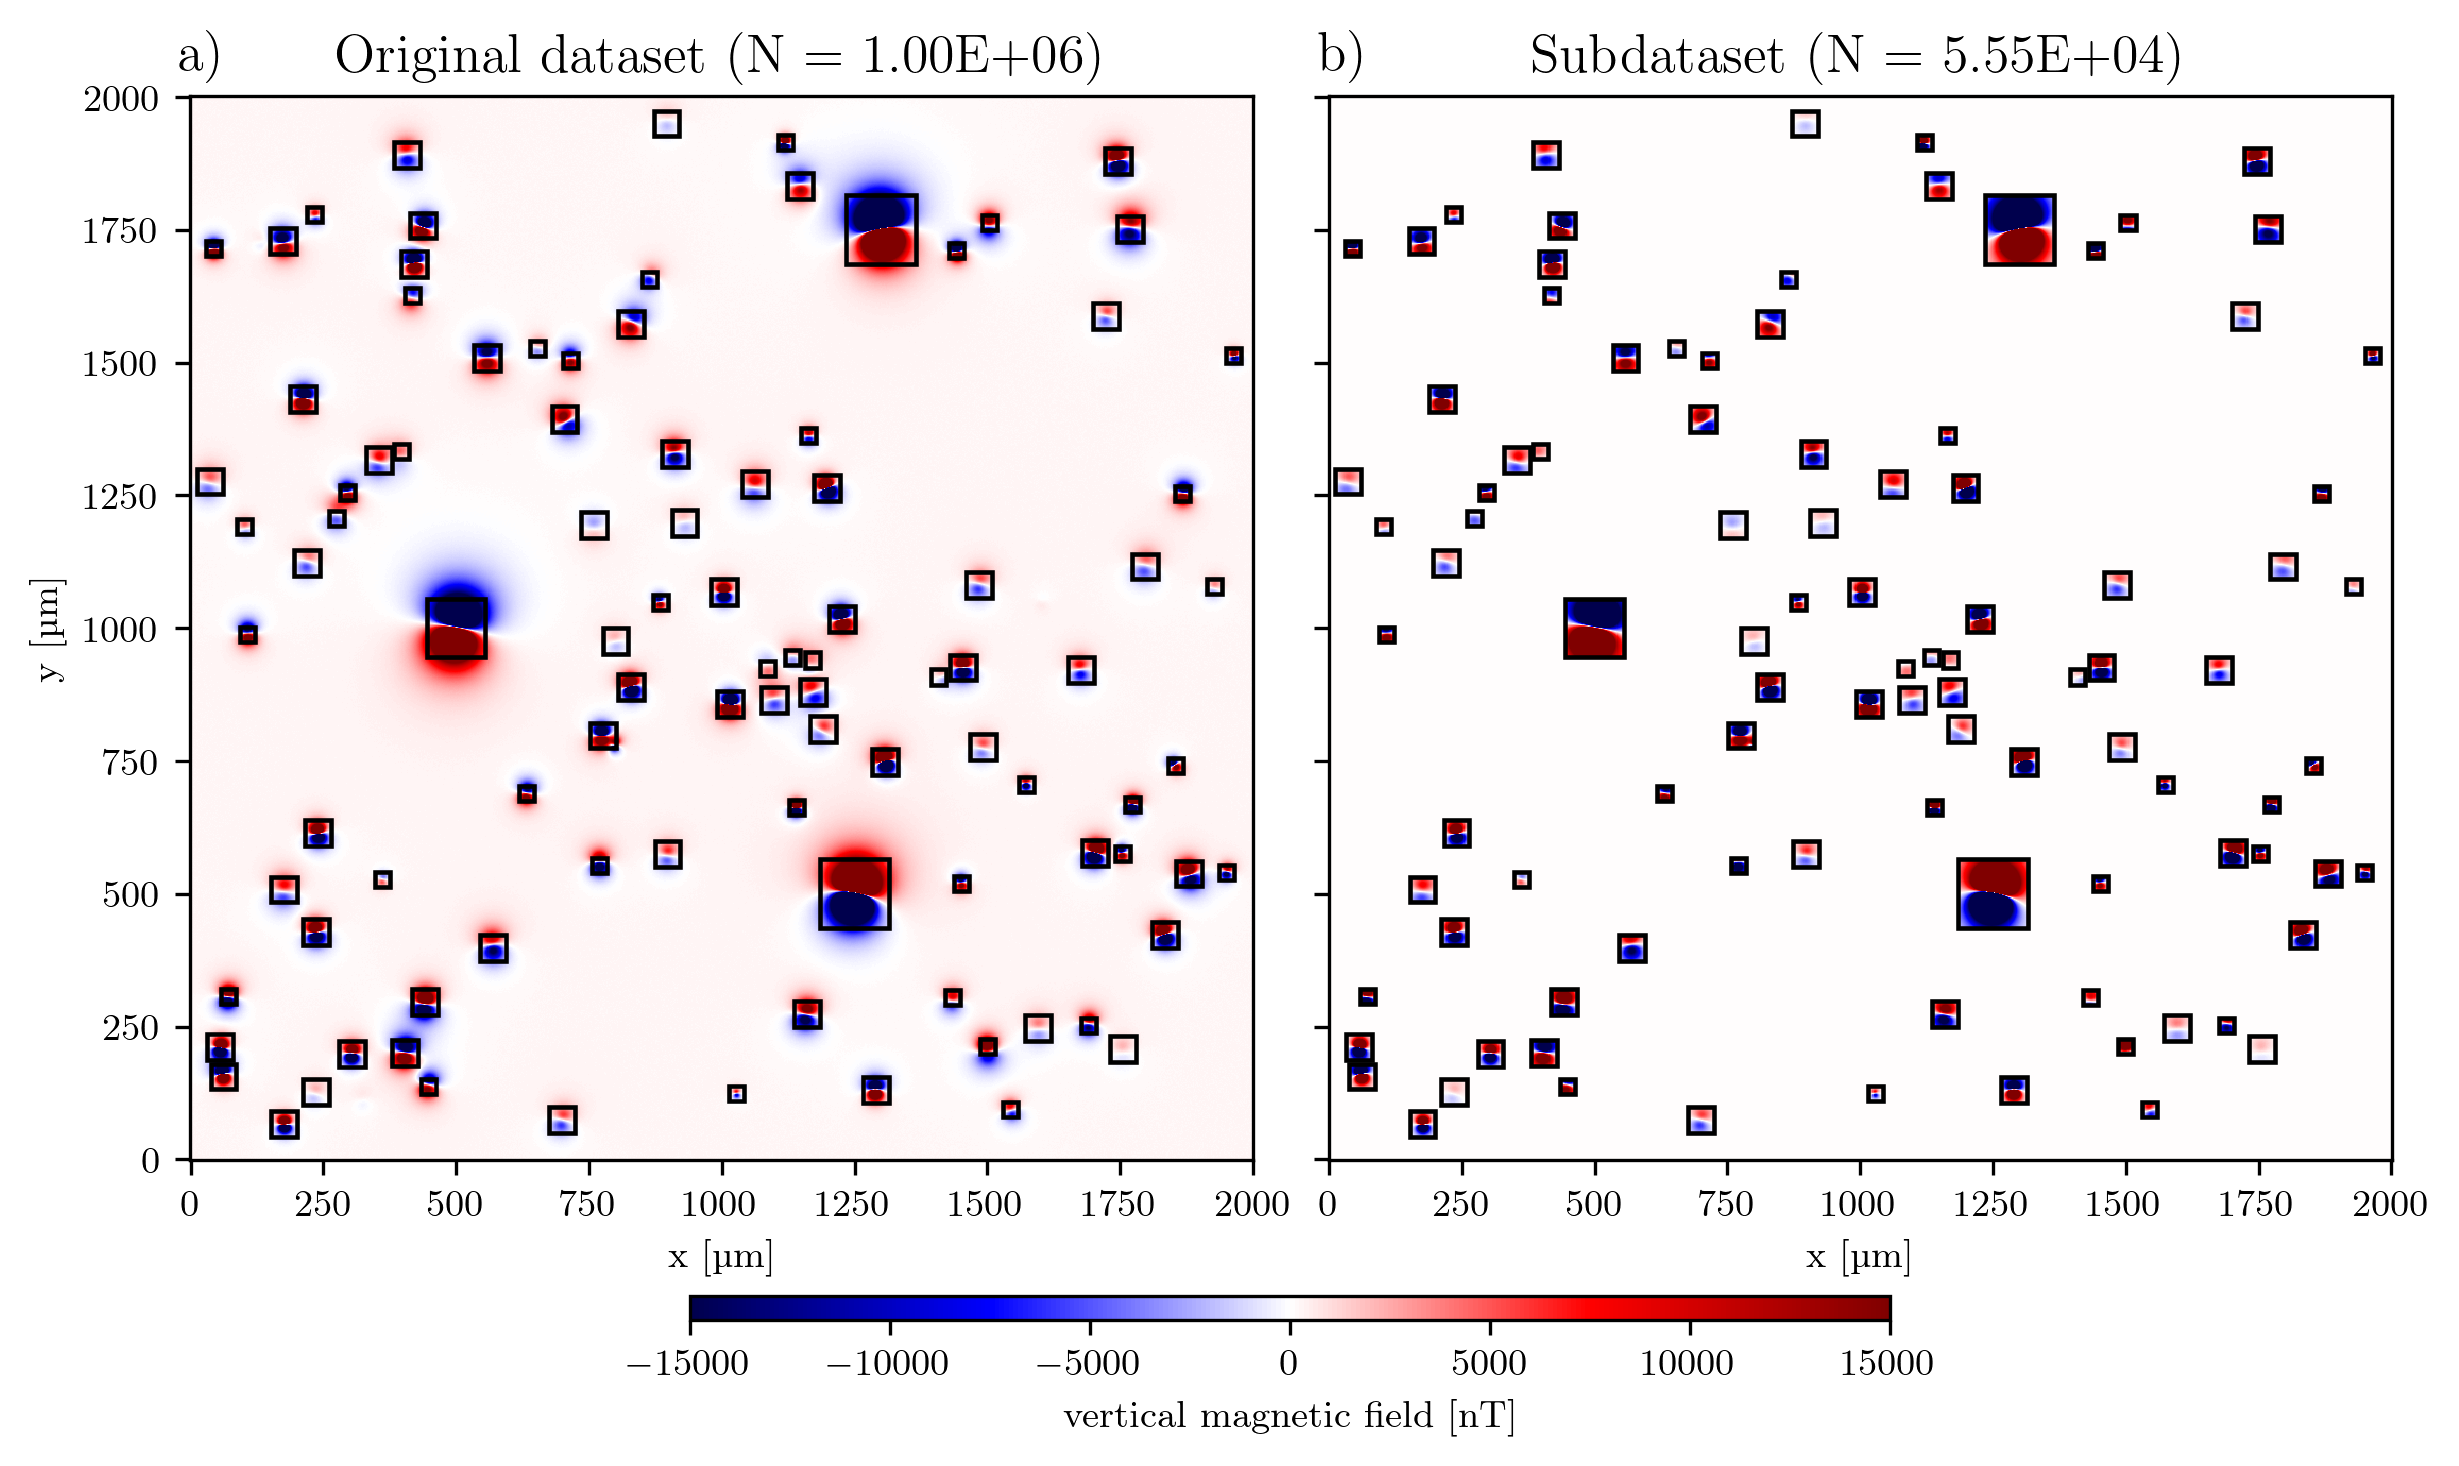
\includegraphics[width=1\linewidth]{figures/methodology.png}
  \caption{
    Addressing computational challenges in magnetic microscopy with extensive datasets.
    a) Complete synthetic dataset featuring all N observation points including areas lacking relevant information.
    b) Streamlining data through pre-selected windows reduces the dataset size for inversion, ensuring efficiency without compromising final results.
      }
  \label{methodology}
\end{figure}

%%%%%%%%%%%%%%%%%%%%%%%%%%%%%%%%%%%%%%%%%%%%%%%%%%%%%%%%%%%%%%%%%%%%%%%%%%%%%%%

\section{Application to Synthetic Data}

As mentioned earlier, this study aims to deal with the mutual interference between the magnetic sources. The proposed methodologies were applied to two sets of complex synthetic data to assess the algorithm's performance. The datasets were designed to evaluate the methodology under different conditions and the inversion workflow was tested for its efficiency in the presence of interfering sources for further comparison with the methodology proposed by the authors. These scenarios are similar to the "Applicability to Real-World Scenarios" showcase by \citet{Souza-Junior2023b}. 

\begin{enumerate}
\item \textbf{Method validation with interfering sources:}
The first model scenario features several dipole sources with different moment magnitudes, inclinations, and declinations clustered around two stable directions. The vertical magnetic field ($b_z$) generated from these sources is corrupted by both low and high-frequency noise, simulating real-world magnetic microscopy data. 

\item \textbf{Shifted magnetic field acquisition:}
The second model replicates the conditions of the first scenario, maintaining the same simulation parameters for the sources. However, in this case, the magnetic field data undergoes a constant positive shift to simulate the acquisition process in magnetic microscopy with a shifted baseline. This scenario provides insights into the algorithm's robustness and accuracy when faced with a systematically shifted magnetic field, as encountered in certain microscopic magnetic data acquisition setups.
\end{enumerate}

\subsection{Method validation with interfering sources}

We analyze how the method works by simulating a complex scenario containing 103 magnetic sources randomly distributed across the imaged area of a synthetic thin section measuring $\qty{2000}{\um} \times \qty{2000}{\um}$. The synthetic $b_z$ data were generated on a regular grid with a spacing of $\qty{2}{\um}$ and a $\qty{5}{\um}$ sensor-sample distance. To make the simulation more realistic, we intentionally incorporated a high-frequency pseudo-random noise, with a zero mean and a standard deviation of $\qty{50}{\nano\tesla}$, as well as low-frequency noise. 

In real ferromagnetic particles, the Natural Remanent Magnetization (NRM) exhibits individual variations but tends to align with the inducing field direction. To capture this variability in our synthetic data, we sampled the dipole moment directions from two pseudo-random Gaussian distributions. The first group of sources ($M = 70$) was sampled from a distribution with a mean of $D = \ang{0}$ and $I = \ang{0}$, with a standard deviation of $\ang{10}$. The second group of sources ($M = 30$) was sampled from a distribution with a mean of $D = \ang{180}$ and $I = \ang{0}$, also with a standard deviation of $\ang{10}$. These sources have distinct depths (between 1 and $\qty{20}{\um}$) and magnetic moment intensities (from $10^{-14}$ to $\qty{e-12}{\ampere\m\squared}$). Additionally, to further emulate the complexities observed in real data measurements, we manually introduced three deep-seated sources with higher dipole moments ($5 \times 10^{-11}$). 

We solved the inversion for this synthetic data using both the standard method \citep{Souza-Junior2023b} and the proposed interfering sources methodologies. A summary of the comparison between the classic Euler method and the iterative approach revealed noteworthy results in the context of the analysis of the provided synthetic data. Upon applying the iterative Euler deconvolution method, a significantly enhanced precision in detecting and positioning magnetic sources emerged when compared to the classic Euler method. Figure~\ref{euler1}a illustrates the detected sources, showcasing the algorithm's effectiveness in identifying regions of interest. Figures ~\ref{euler1}b and ~\ref{euler1}c show the results obtained by the standard and iterative Euler methods, respectively. It becomes evident that the iterative method yields more accurate and refined estimates. This increase in accuracy is crucial, especially in scenarios where stronger magnetic sources can distort the outcomes. However, it is important to note that the enhanced precision with the iterative method comes at the cost of increased computational time, presenting a trade-off between superior results and computational efficiency.


\begin{figure}[tb!]
  \centering
  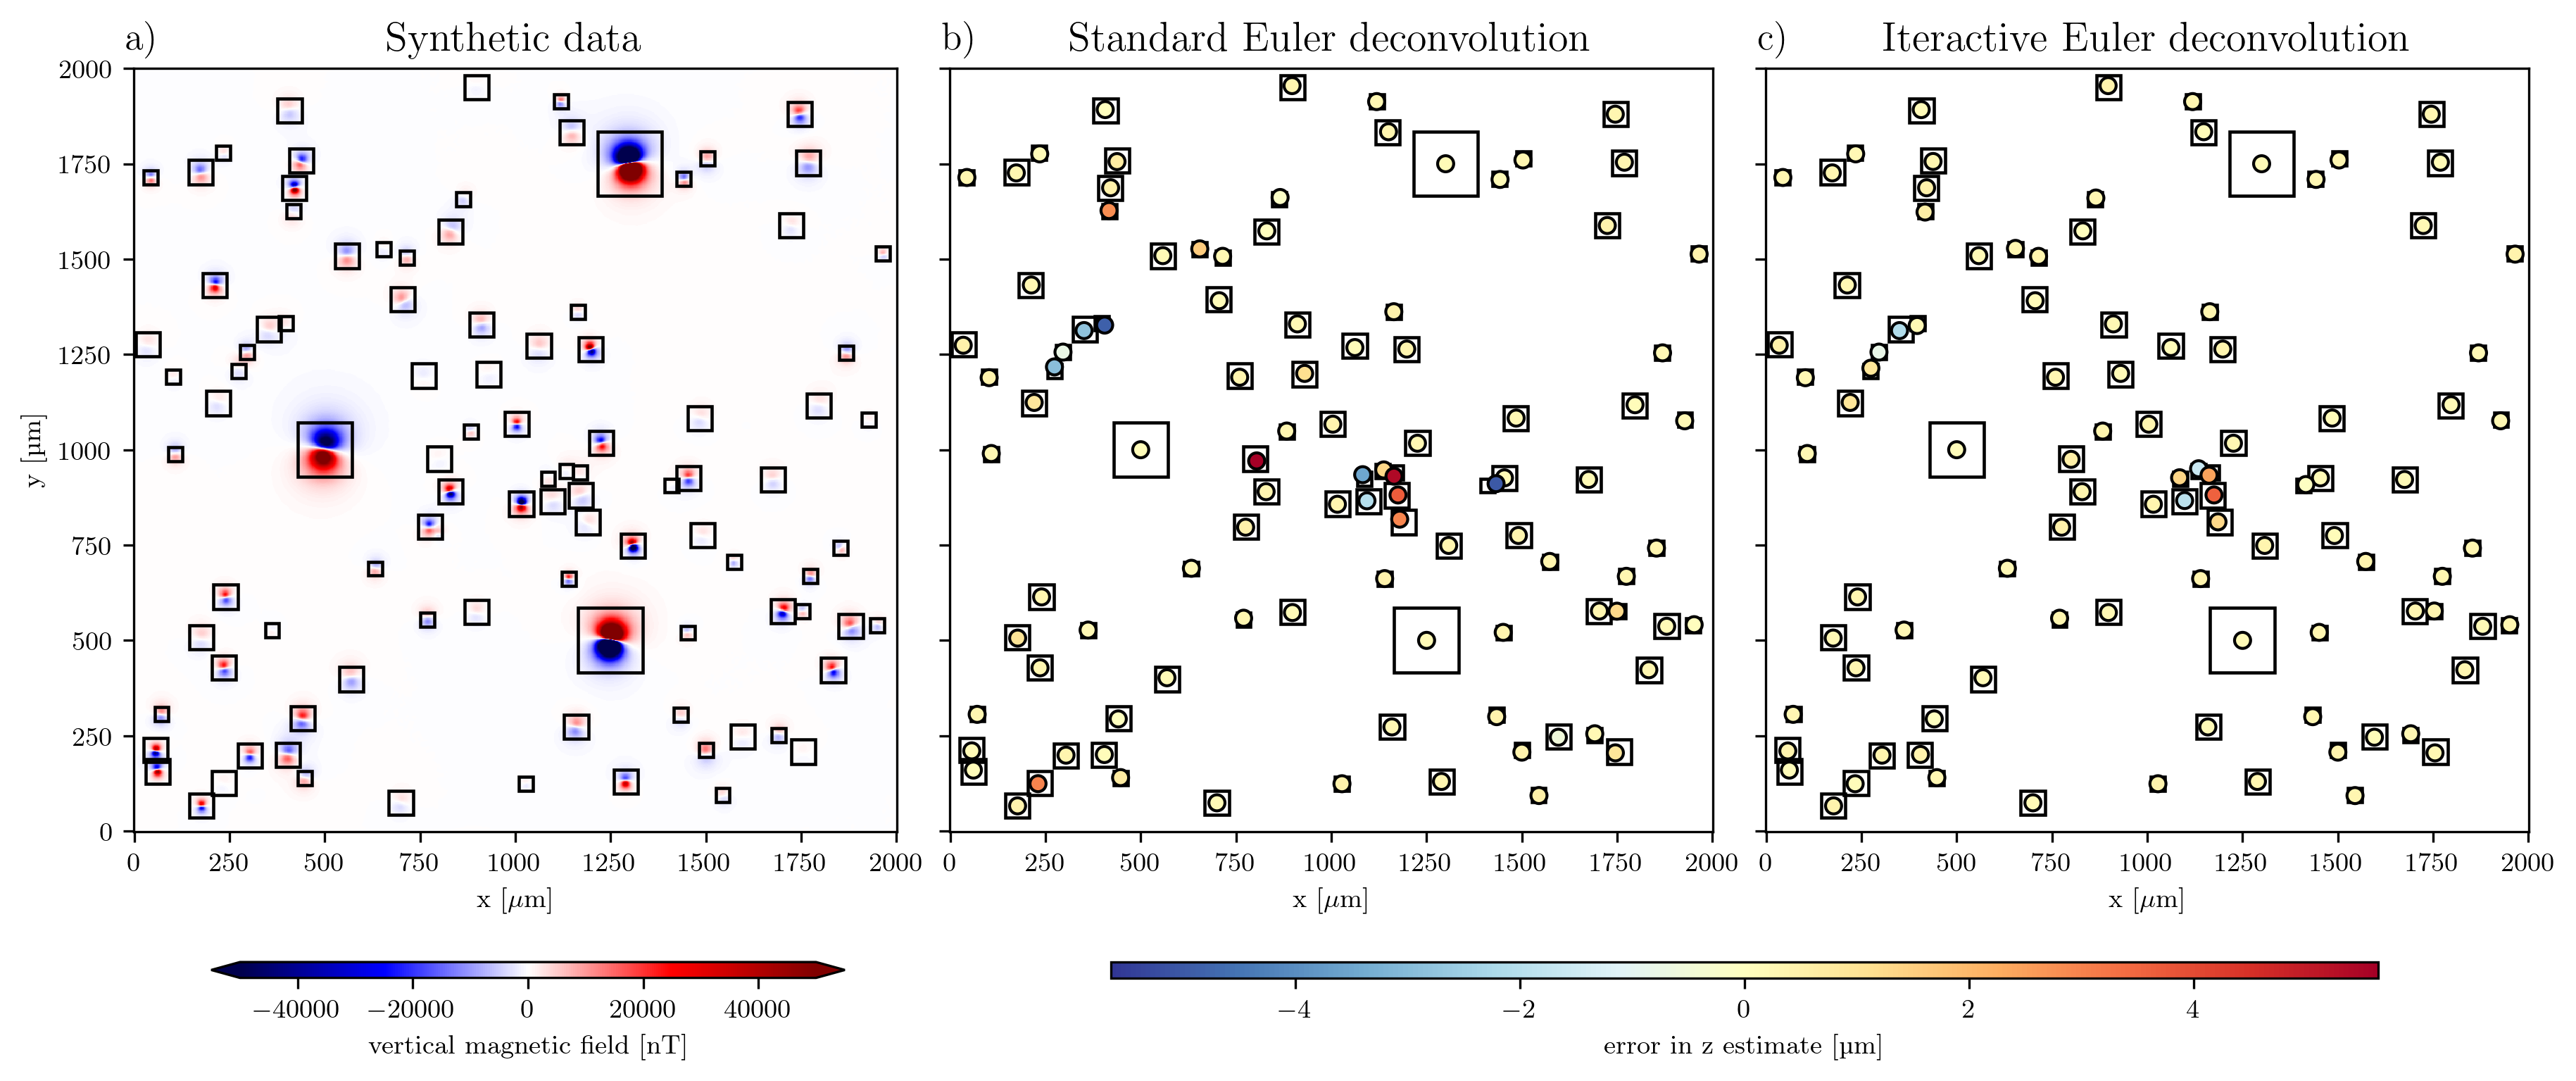
\includegraphics[width=1\linewidth]{figures/euler-comparion-1.png}
  \caption{
    % Addressing computational challenges in magnetic microscopy with extensive datasets.
    % a) Complete synthetic dataset featuring all N observation points including areas lacking relevant information.
    % b) Streamlining data through pre-selected windows reduces the dataset size for inversion, ensuring efficiency without compromising final results.
      }
  \label{euler1}
\end{figure}

bla bla bla bla

\begin{figure}[tb!]
  \centering
  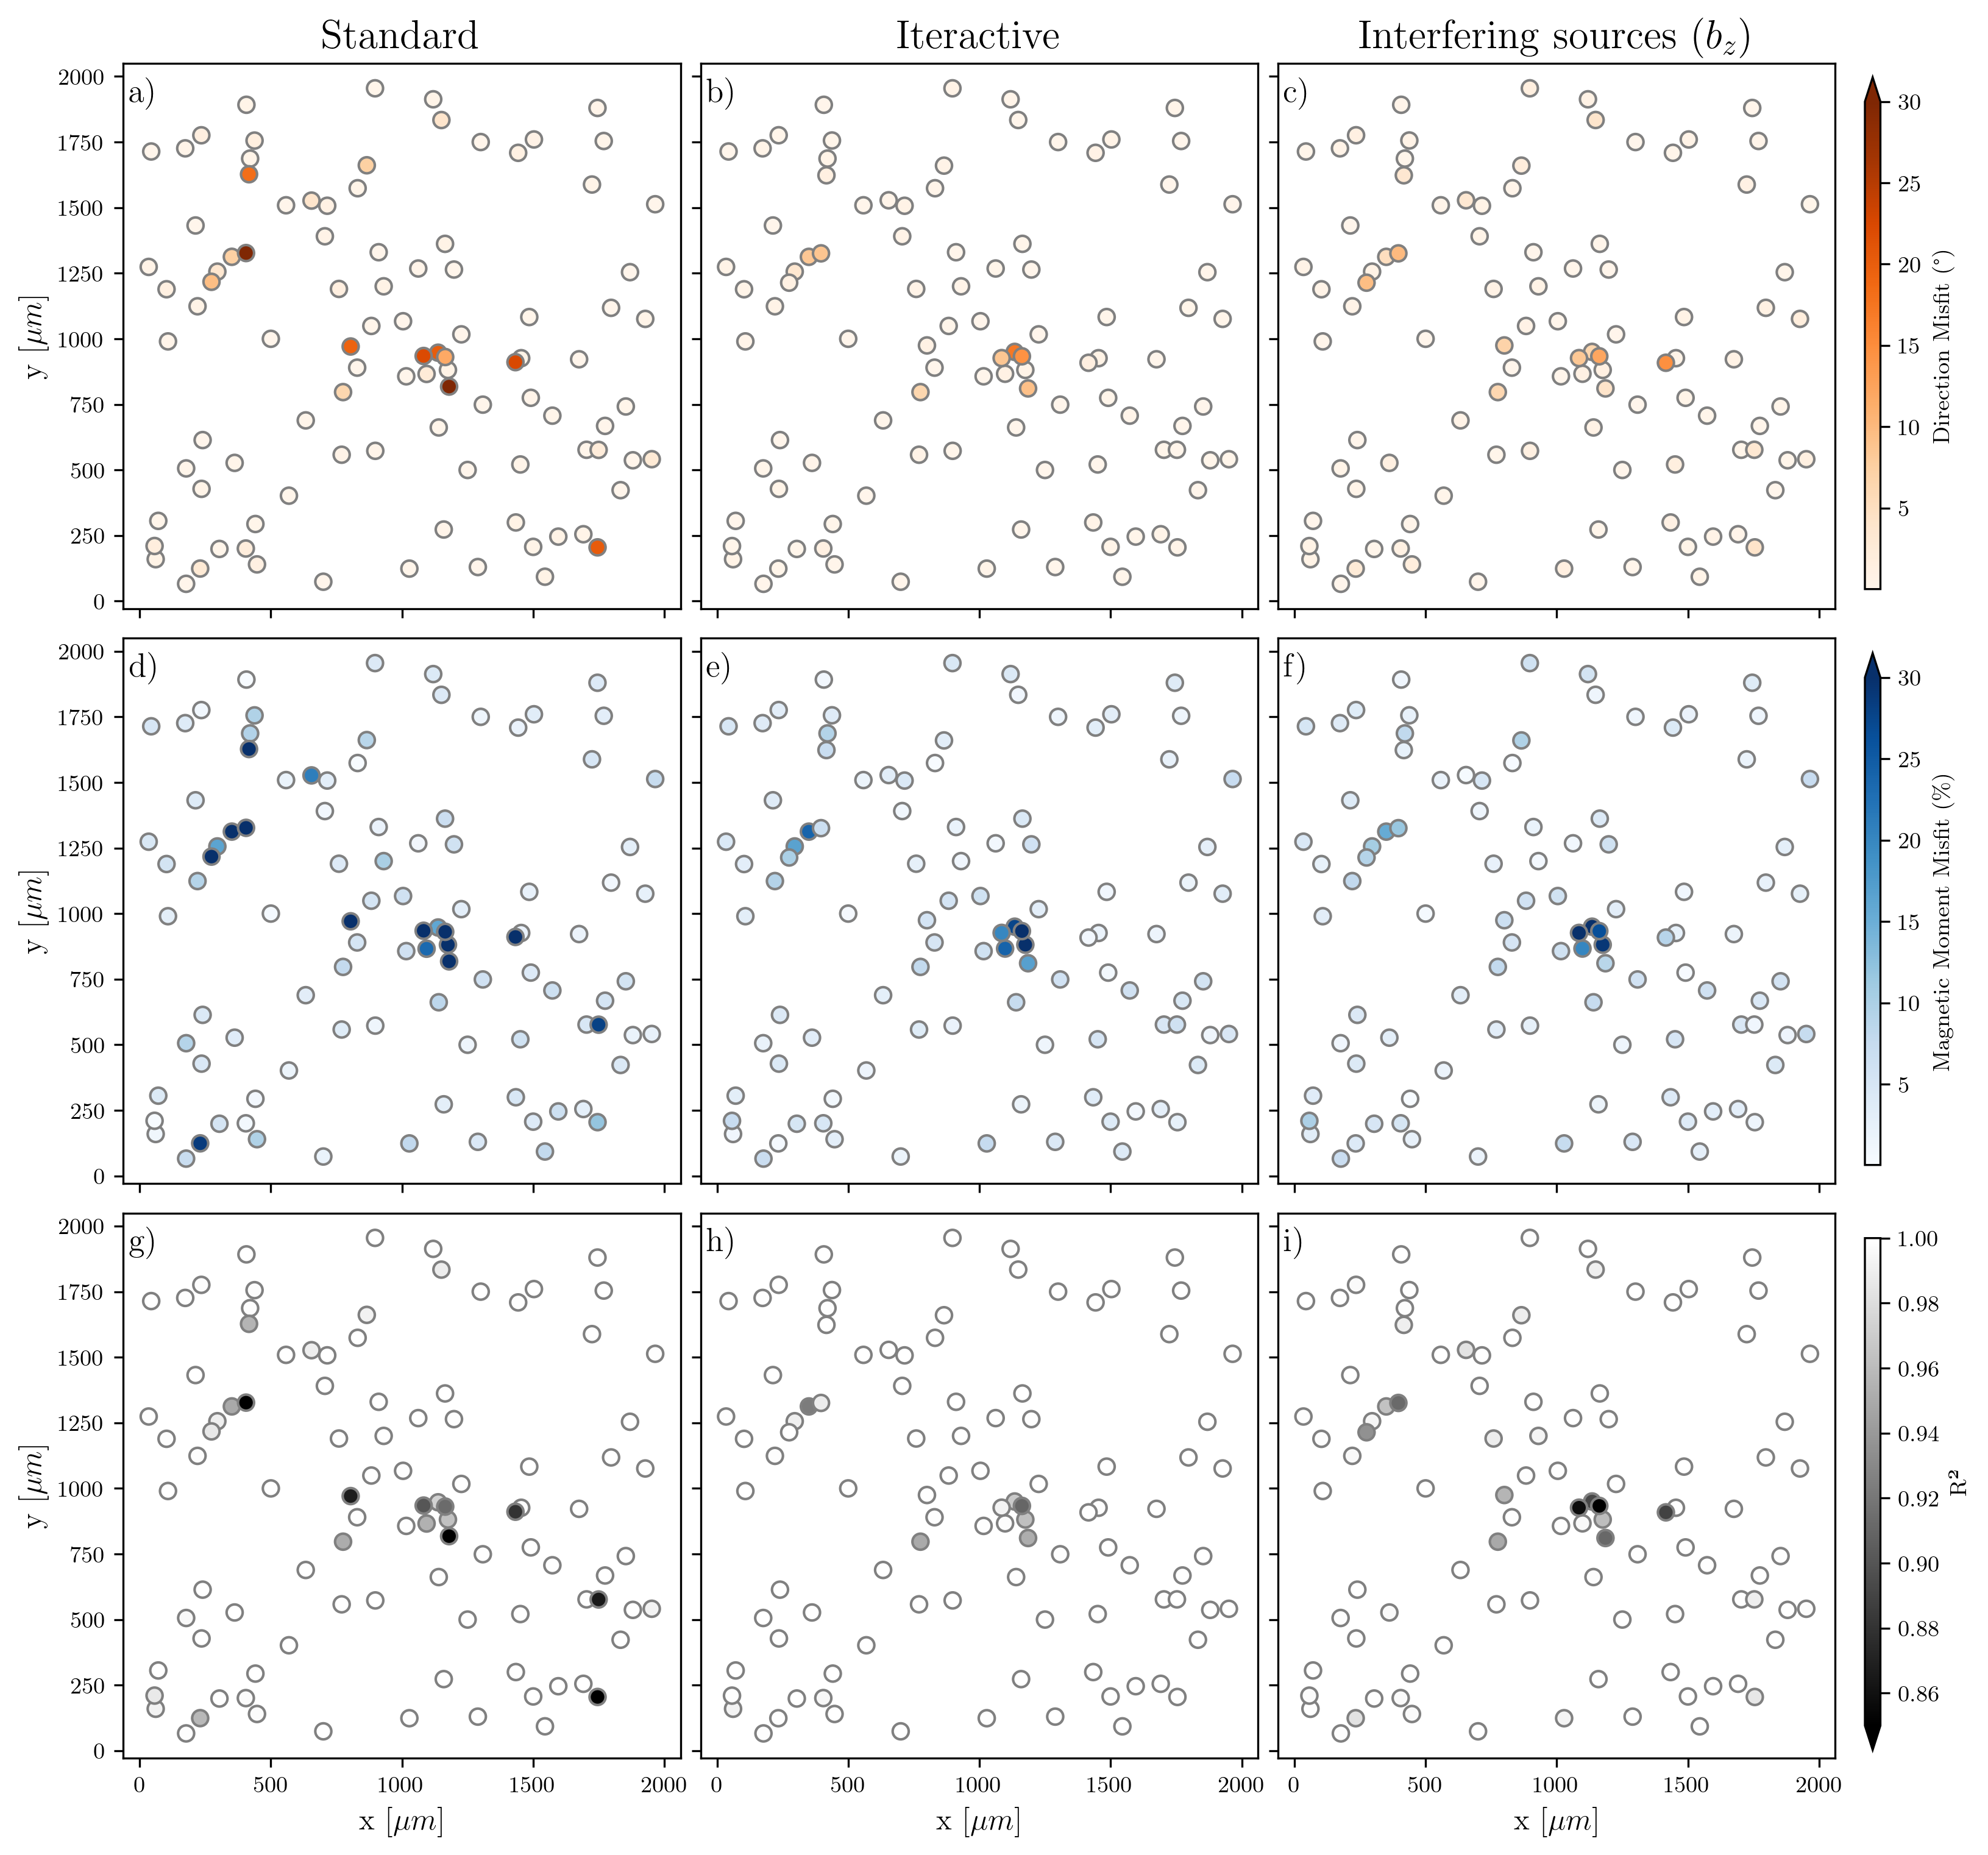
\includegraphics[width=1\linewidth]{figures/inversion-comparion-1.png}
  \caption{
    % Addressing computational challenges in magnetic microscopy with extensive datasets.
    % a) Complete synthetic dataset featuring all N observation points including areas lacking relevant information.
    % b) Streamlining data through pre-selected windows reduces the dataset size for inversion, ensuring efficiency without compromising final results.
      }
  \label{inversion1}
\end{figure}




\subsection{Shifted magnetic field acquisition}

bla bla bla

In all the synthetic and real data analyzed in this paper, the vertical derivatives were computed using the central finite difference equation (Equation x).

%%%%%%%%%%%%%%%%%%%%%%%%%%%%%%%%%%%%%%%%%%%%%%%%%%%%%%%%%%%%%%%%%%%%%%%%%%%%%%%
\section{Discussions}


%%%%%%%%%%%%%%%%%%%%%%%%%%%%%%%%%%%%%%%%%%%%%%%%%%%%%%%%%%%%%%%%%%%%%%%%%%%%%%%
\section{Conclusion}



%%%%%%%%%%%%%%%%%%%%%%%%%%%%%%%%%%%%%%%%%%%%%%%%%%%%%%%%%%%%%%%%%%%%%%%%%%%%%%%
\section{Open research}

The Python source code used to produce all results and figures presented here, as well as supplemental figures and Jupyter notebooks, are available from \citet{sourcearchive}, which can also be found on \url{https://github.com/\GitHubRepository} under the MIT and CC-BY licenses.
The QDM magnetic microscopy data are available
from \citet{janinedata} under the CC-0 license.

The image re-scaling and blob detection through the Laplacian of Gaussian
method were performed with the scikit-image library \citep{VanderWalt2014}.
We also used matplotlib \citep{Hunter2007} and mplstereonet \citep{mplstereonet}
for generating figures and stereograms.
Basic calculations were performed using Numpy \citep{Harris2020} and Scipy
\citep{2020SciPy-NMeth}.
Verde \citep{verde2018} was used to generate data grids.
Upward continuation was performed using Harmonica \citep{harmonica2020}.
The Choclo library \citep{choclo2022} provided kernel functions used in the
forward and inverse problems.
The Numba just-in-time compilation library \citep{lam2015numba} was used to
speed-up calculations.
Lastly, the xarray library \citep{hoyer2017xarray} offered a fast and powerful
tool for working with multi-dimensional datasets allowing an easy way of data
visualization and extraction with advanced indexing techniques.



%%%%%%%%%%%%%%%%%%%%%%%%%%%%%%%%%%%%%%%%%%%%%%%%%%%%%%%%%%%%%%%%%%%%%%%%%%%%%%%
\section{Acknowledgements}

We are indebted to the developers and maintainers of the open-source software
without which this work would not have been possible.
This research was supported by
grant 162704/2021-6 from the Conselho Nacional de Desenvolvimento Científico e Tecnológico (CNPq),
grant 2021/08379-5 from the Fundação de Amparo à Pesquisa do Estado de São Paulo (FAPESP),
grant PRPI 22.1.09345.01.2 from Universidade de São Paulo,
and grant IES\textbackslash{}R3\textbackslash{}213141 from the Royal Society.
The opinions, hypotheses, and conclusions or recommendations expressed in this
material are the responsibility of the authors and do not necessarily reflect
the views of FAPESP.
